\documentclass[11pt]{article}

\usepackage{deauthor}
\usepackage{times}
\usepackage{graphicx}
\usepackage{authblk}
\usepackage{hyperref}

\usepackage[usenames,dvipsnames,svgnames]{xcolor}

\newif\ifdraft
%\draftfalse
\drafttrue
\ifdraft
\newcommand{\ian}[1]{\textcolor{Red}{[Ian: #1]}}
\else
 \newcommand{\ian}[1]{}
\fi


\graphicspath{{figs/}}

\title{Plenario: An Open Data Discovery and Exploration Prototype}

\author[1,2]{Charlie Catlett}
\author[2,1]{Brett Goldstein}
\author[2]{Jonathan Giuffrida}
\author[1]{Robert Mitchum}
\author[1]{Alessandro Panella}
\author[3]{Derek Eder}
\author[3]{Eric van Zanten}
\affil[1]{Urban Center for Computation and Data, Computation Institute of the University of Chicago and Argonne National Laboratory}
\affil[2]{Harris School of Public Policy, University of Chicago}
\affil[3]{DataMade, LLC}

%\author{Me}

%IAN: Title doesn't mention city or geospatial, which seem to me to be two critical aspects of the system.


\begin{document}
\maketitle

\begin{abstract}
The last decade has seen rapid growth in the release of open data by government bodies and other public institutions of all sizes. Today, hundreds of open data portals, hosting thousands of data sets, present researchers, policymakers, service providers, journalists, and the general public with enormous opportunities to better understand the dynamics and processes of cities and ultimately to develop solutions to improve the lives of residents. However, any individual seeking to seize these opportunities quickly finds that discovering and exploring the open data relevant to any specific inquiry is extremely difficult. In this context, we introduce Plenario, a platform designed to provide two key capabilities to any individual, even those without prior knowledge or expertise in open data : (a) \emph{discovery} of data associated with a place and window of time, and (b) \emph{exploration} of such data to identify potential interdependencies between relevant data sources. These capabilities are realized by a 
The resulting data sets are intended to support deeper analysis with advanced tools and applications; thus users can refine, combine, and export data sets. In order to effectively support discovery of open data, Plenario includes tools for administrators and users to specify data sets to be imported and kept updated. The architecture of the system involves a cloud-based geospatial database, implemented as open source and leveraging a number of open source components. The use of the Amazon Web Services commercial cloud infrastructure enables any organization to replicate Plenario and populate a local instance with data of interest. Cloud infrastructure will also enable instances of Plenario to readily scale to support thousands of data sets from hundreds of sources. In this paper we present the context and objectives of the Plenario platform, its architecture and implementation, a discussion of lessons learned through Plenario instances for specific user communities, and an outline of plans for future work on Plenario based on these lessons.
\end{abstract}

\newpage

\section{Plenario Context and Objectives: Open Data Discovery and Exploration}
\label{sec:context-objective}
Over the past decade, cities worldwide have adopted new policies encouraging or even mandating broad public release of a wide range of municipal and federal data\ian{Can a city release federal data?}. 
Cities such as Chicago, San Francisco, New York City, Barcelona, and Glasgow have launched online data portals containing datasets on a multitude of topics.
Worldwide, we see the establishment of hundreds of open data portals and the release of tens
%Thomas Levine (http://thomaslevine.com/\_\_33\_\_/socrata{}-summary/) counts 88k Socrata datasets alone. Need to cite or obvious from {}``hundreds{}'' times {}``hundreds{}'' in citation 1?
%Jonathan Giuffrida
%February 8, 2015 4:22 PM
 of thousands of data sets \cite{maksimovic_2011}.  Many of these portals include frequently updated data on crime, city contracts, business licenses, food safety inspections, service requests, traffic, energy usage, schools, and other data of importance to residents and researchers. This data, released in a spirit of transparency, public access to city information, and collaboration with the community, has already been used for a wide range of purposes, many unanticipated. Software developers\ian{It said ``developers," I assume that this meant software developers, not real estate developers?} have used these new data sources to build new applications. Journalists have used them to research stories and watchdog government activities. Researchers in sociology, education, economics, behavioral sciences, and other disciplines have launched new data-driven research projects. And policymakers have used new data sources to engage the public on new strategies and initiatives. 
 
While this first wave of open data produced undeniable benefits, several issues prevent the movement from reaching its full potential. Most importantly, ``open'' does not always mean ``accessible.'' Finding relevant data in the many open data portals is largely a manual exercise requiring a high degree of experience and familiarity with portal technologies and their interfaces. Concurrently, most datasets are released in file formats and structures that make integration and analysis time-consuming for skilled data analysts, and effectively out of reach to the general public. Even the most advanced portals release most datasets in the form of massive spreadsheets or tables, leaving the user with the burden of visualizing, mapping, and combine those large datasets. Further, many of the cyberinfrastructure technologies and tools used to make this data available were designed primarily to support the analysis of individual datasets rather than exploring relationships among many datasets. These technical hurdles make asking simple questions, such as ``What data sets are available for the block on which I live?'' or ``What is the relationship between air quality and health in my city?'' immensely challenging. Simply put, these challenges mean that many important questions remain unexplored and much of the opportunity of open data remains to be realized.
\ian{Perhaps we could say simply that while data was ``released," what this meant in practice was that data was dumped without any descriptive metadata, in a wide range of formats, etc.--thus unintelligible to anyone lacking private knowledge.}

This problem of combining datasets to find insight exists within city government as well and has inspired novel solutions in the recent past. 
One such project, WindyGrid~\cite{windygrid}, was developed for internal use by the City of Chicago in anticipation of hosting the 2012 NATO Summit. It organizes disparate datasets (internal to the city as well as public sources such as social networks) by their space and time coordinates using geospatial database technology, allowing city officials to discover and explore multi-dimensional, real-time information about different areas of the city. This integration supports much more informed and effective deployment and coordination of services, including emergency responses. After the summit, the city continued using WindyGrid, expanding its use by adding tools to analyze and improve city services.

In the same time period, the University of Chicago's Urban Center for Computation and Data (UrbanCCD) \cite{urbanccd} organized the Urban Sciences Research Coordination Network (US-RCN) \cite{us-rcn} to bring together scientists, policymakers, social service providers, and others to explore the use of open data for social science research. Disciplines represented in US-RCN range from sociology to economics; questions studied range from healthcare to education, crime, and employment. Interaction within this diverse community, along with lessons learned designing and using WindyGrid, revealed that a critical need for many data-enabled inquiries is to be able to easily find and access data about a particular place and for a particular window of time.

Such inquiries tend to follow a common workflow, as shown in Figure \ref{fig:plenario-workflow}(a). This workflow relies on the investigator having, first of all, intimate knowledge about what data sets are available, and from what sources, as well as familiarity with the portal technologies and their internal search, refinement, and export functions. 
Then, once relevant datasets have been retrieved, the diversity of spatial and temporal resolution and organization of data from different sources means that the
investigator requires additional expertise, and must devote considerable time, to their examination, refinement, and aligning and merging. The result is that effectively using open data requires both considerable knowledge and expertise in navigating and finding data as well as resources to evaluate and prepare the data.

\begin{figure}
	\centering
	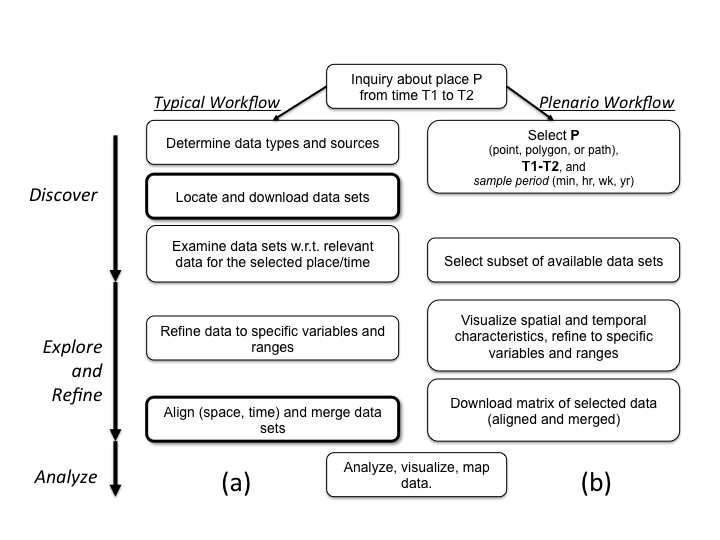
\includegraphics[scale=.5]{plenario_workflow.png}
		\label{fig:plenario-workflow}
	\caption{Two different approaches to open data discovery, exploration, and analysis: (a) the traditional, expertise- and labor-intensive approach and (b) the space- and time-based exploration process supported by Plenario.\ian{I don't think my revised caption is quite right, but I think it is better. Figure could be improved. Color the two sides to distinguish better?
	Add arrows between boxes to show flow? Why do two boxes on the left have thicker lines? Maybe show iteration between select and visualization boxes on right via circular arrow?}}\ian{I moved captions below figures, as that is the conventional place to put them.}
\end{figure}

The Plenario project began with a hypothesis that for open data to have truly transformative impact, it must be accessible to non-data scientists, by individuals without familiarity with the growing collection of open data portals (or their user interfaces). Above all, it must be possible to explore data quickly, without first investing weeks or months in data preparation. Plenario is a prototype platform developed to test this hypothesis by bringing many open data sets together, integrating them, and presenting a map-based interface for users to discover data sets relevant to a particular place over a period of time, and to examine the potential for interdependencies among those data sets.
\ian{Should you say here what you have learned so far from this experiment?}

\subsection{Plenario: An Overview}
Plenario exploits the fact that the vast majority of open data portals are implemented using one of just two platforms: the Socrata Open Data API (SODA) \cite{socrata} or Comprehensive Knowledge Archive Network (CKAN) \cite{ckan}. Each platform offers various internal search capabilities and visualization tools. Importantly for our purposes, each also provides an API for accessing and downloading data, and thus supports external application development. Yet at present there is no federation of these platforms or cross-platform search capabilities\ian{Not clear whether you mean lack of federation between the two platforms, or between the hundreds of portals that are based on those platforms.}. In part the lack of search capabilities reflects the diversity of the data, from text to spreadsheets to shapefiles, and a lack of clarity as to how best to search large collections of sources---keyword? Full text? Based on interactions with the US-RCN community and the experience with WindyGrid in the City of Chicago, we designed Plenario to support place and time inquiries. Thus, we use a map interface with time specifications to implement search. The resulting user interface replaces the first two steps in typical workflows---the ``Discover'' phase shown in Figure \ref{fig:plenario-workflow}.\ian{How does Plenario then relate to the platform APIs? Are you saying that Plenario is a frontend to different SODA and CKAN portals? Or is the first past of this paragraph unrelated to the second part?}

\ian{It seems to me that there is are important points here that are not as clearly presented as they could be.
A key point is that before using open data for a particular region, the user must do two things: (1) find relevant available datasets, and (2) subset/extract/transform
from those datasets to get just what is needed for that region. 
\\
There are then two problems with the traditional approach. First, (1) is difficult because of (a) a lack of suitable descriptive metadata, and perhaps 
also because (b) the user can't easily find which datasets overlap with the region of interest. Second, (2) is not supported at all: it is left entirely up the the user.
I feel that these critiques are made rather circuitously.  The text doesn't really say 1(a) explicitly, and doesn't mention 1(b) at all. (2) is mentioned, but again could be more direct.
\\
Turning to the Plenario approach, I get that one big advantage is that (2) is automated: Plenario will extract just the data that pertains to a region.
I am less clear about (1). How does Plenario make search easier? It it because it integrates additional metadata [1(a)]? Or is it because of 1(b)?
\\
One more thing that I am unclear about: I imagine that once data has been extracted for a region, there are a set of challenges relating to different data formats, different
grid systems, the need to apply spatial statistics on funny shaped regions, etc. Does Plenario help with those things?}

Beyond the need for search, open data sources are diverse with respect to their spatial and temporal organization, resolution, units of measure, and other factors. Plenario imports data sets and integrates them into a single geospatial database, performing the alignment and merger of the data sets, eliminating the need for the user to do so, as shown in the ``Explore and Refine'' phase of Figure \ref{fig:plenario-workflow}. Moreover, the Plenario workflow does not rely on user knowledge to determine where relevant data might exist\ian{I don't understand the point being made here. Is the point here that: (a) user knowledge is not needed because Plenario loads data in from lots of different portals, via the use of open APIs? (b) user knowledge is not needed because the space/time-based search reduces the number of datasets that a user needs to consider? (c) Plenario adds more descriptive metadata, making search easier?}. Nevertheless, Plenario provides a web form for requesting the import of additional data sources. 

Plenario thus enables the simpler, more intuitive workflow shown in Figure \ref{fig:plenario-workflow}(b).
Note the new open data discovery capability and the automation of several of the most costly steps in the traditional workflow of Figure \ref{fig:plenario-workflow}(a)---notably the ``Locate and download'' and ``Align and Merge'' steps. Thus, instead of searching for and combing through a multitude of potential open data sources and datasets to find data of interest for a particular location, the user specifies geographical boundaries and instantly receives all of the data available for that location (Figure \ref{fig:plenario-search-example}). The labor-intensive work of combining and aligning the various spatial and temporal attributes of data sets has already been performed as part of the data import functions of Plenario, significantly shortening the path from question to discovery.

Plenario is not intended to replace full-featured data analysis tools. 
Nevertheless, we find that users often want to check high-level data features before committing to download data for local analysis. 
Thus, we have incorporated basic data visualization, mapping, and time series creation capabilities into the Plenario prototype.
As shown in Figure~\ref{fig:plenario-dataset-vew}, when Plenario lists a data set in response to a user query it shows not only basic information and links to provenance and meta data, but also a simple time series graph. Such graphs can help users determine whether a particular dataset might provide relevant information for a particular temporal query. Once a dataset has been identified as shown in Figure~\ref{fig:plenario-dataset-vew}, the user can then select it and request a map-based view to examine the data's  spatial density. This view includes aggregation-level controls that permit the user to modify the aggregation density from 100 meters to 1 kilometer\ian{Unclear: ``between" those two numbers, or are they the only two supported?}. Finally, the user can further refine the view of a selected data set by specifying fields and values or ranges of interest. These tools all serve to enable the user to determine a data set's relevance to their questions before exporting them for further analysis.

The Plenario platform not only helps individual researchers: it also helps avoid duplication of effort by providing a space in which users can collaborate on cleaning data and exploring datasets in more sophisticated ways\ian{Not sure what that last bit means.}. 
A key point is that each dataset only needs to be imported once, after which it can be by anyone---or, in the case of sensitive datasets, by all authorized users.
Similarly, all results of data cleaning are available for all users.\ian{It isn't clear to me how data cleaning fits into the picture. How is it done?}

\section{Plenario Architecture and Implementation}
The Plenario software platform is open source and available at GitHub \cite{plenario-github}. We have designed the software to be hosted on the Amazon Web Services commercial cloud. This approach facilitates replication in several important ways. First, governments and other organizations can readily create an instance of Plenario for their use, potentially including both open and internal data. Second, organizations can provide open data for integration into an existing Plenario instance, such as the one operated by the University of Chicago at {\tt http://plenar.io}. They can then use Plenario's analysis tools and API to power their own applications. The architecture allows data providers to choose which datasets are available to the public and which should remain ``closed,'' available only for internal use for authorized users. The San Francisco Plenario instance, detailed below, is being used to explore functions for aggregating sensitive data prior to presenting to the end user.\ian{It seems to me that this text mixes together a few somewhat unrelated issues. (1) ``A fundamental design assumption is that there will be multiple, perhaps many, Plenario instances." This is important because it allows for private data, etc. (2) ``We assume AWS hosting." This might be for two reasons: (a) it presumably makes it easy for users without local IT expertise to stand up an instance; (b) it simplifies our work implementing and supporting the Plenario software, as we can assume a single platform. [On the other hand, it might be a concern for really OCD security types when data is sensitive.] (3) ``Plenario is open source." We don't say why that is important. Is it because it allows others to contribute to it? (It isn't needed for us to share access via AWS.) (4) [Not stated explicitly, but implied--and it seems important.] ``Plenario allows for the administrator of a Plenario instance to control who can access which datasets." [Or are we instead saying that when data is sensitive, the administrator has to create two instances: one for sensitive, one for public? It's not clear.] (5) ``Organizations can contribute data for integration into an existing instance." Not clear why this is mentioned: it doesn't seem to be an architectural feature? Or are there some architectural implications?}

Here we describe the Plenario architecture. We describe, in particular, the following features: (a) data import via an automated Extract-Transform-Load (ETL) builder, (b) integration using a geospatial database, and (c) special cases for common data sets such as weather and census data. In brief, an automated extract-transform-load (ETL) builder imports and inserts each dataset as a table in a PostgreSQL database. The ETL builder includes a specification for update frequency, so that Plenario can update the dataset at the same frequency as the source dataset is updated. Each row in each dataset is represented by a pointer in a single ``Master Table,'' so that all data is indexed on the same spatial and temporal indices\ian{Sounds good, but I am not sure what is meant. Do you interpolate data to a common fixed lat/lon (and temporal) grid? If so, how? Or are you just saying that you use the same coordinate system?} (Figure \ref{fig:flowchart}). The platform then joins each observation to a set of commonly used data sets including sensor and place-based data and exposes the dataset in the relevant API endpoints\ian{What does that mean?}.  The web portal (and other clients) can then access the data via the API.

\subsection[data-import]{Data Import: \textbf{Automated ETL Builder}}
A dataset can be submitted to Plenario simply by providing a URL that links to a publicly available table in CSV format\ian{I switched ``is submitted" to ``can be submitted" because presumably this is not the only mechanism. At least you have said elsewhere that you support non-public data.}. This approach can be used to submit any datasets on a SODA or CKAN platform or self-hosted by the user\ian{I don't see how this can be true. First, do SODA and CKAN APIs support GET access to a CSV file? (And what is the protocol? Is it HTTP?) Second, sort of obvious, but ignorning the protocol issue, this does not support ``any dataset," only CSV tables.}. Plenario's automated ETL builder scans the dataset, infers field types, and checks for common data integrity issues. As Plenario currently focuses on spatio-temporal datasets, the user is then asked to identify which fields correspond to the spatial field(s)\ian{And presumably you need to know the syntax and semantics of these fields?}, temporal field, and unique ID, and how frequently the dataset updates\footnote{Future improvements to Plenario will remove one, two, or all three of these requirements, in some cases: see Section \ref{sec:challenges}}. The user can also add information regarding the dataset's provenance, description, and license if these are not automatically populated (as they are with SODA datasets). 

Following a basic check for URL stability and malware, an ETL worker process begins importing a local copy of the dataset as a new table in the PostgreSQL database. After import, Plenario inserts a row into the Master Table for every row in the new dataset. This new Master Table row contains the dataset ID, the row ID (unique ID), and the spatial and temporal fields. The dataset is then made available via a RESTful API with endpoints\ian{Just to check: these are really distinct endpoints} for raw data, data aggregation by time and space, metadata, and weather-specific data (weather is one of several special case base data sets discussed in Section \ref{sec:commonly-used-datasets}). Tasks are automatically scheduled to update the dataset according to the refresh frequency of the source dataset, using the unique ID (when available: see Section \ref{sec:challenges}) to avoid re-populating the entire table. Multiple datasets can be imported and updated simultaneously using multiple ETL workers.\ian{It seems to me that this discussion of the Master Table is not as clear as it could be. I understand it somehow links everything that is at a single ``point" in space and time, but I don't understand how.}

\begin{figure}
	\centering
	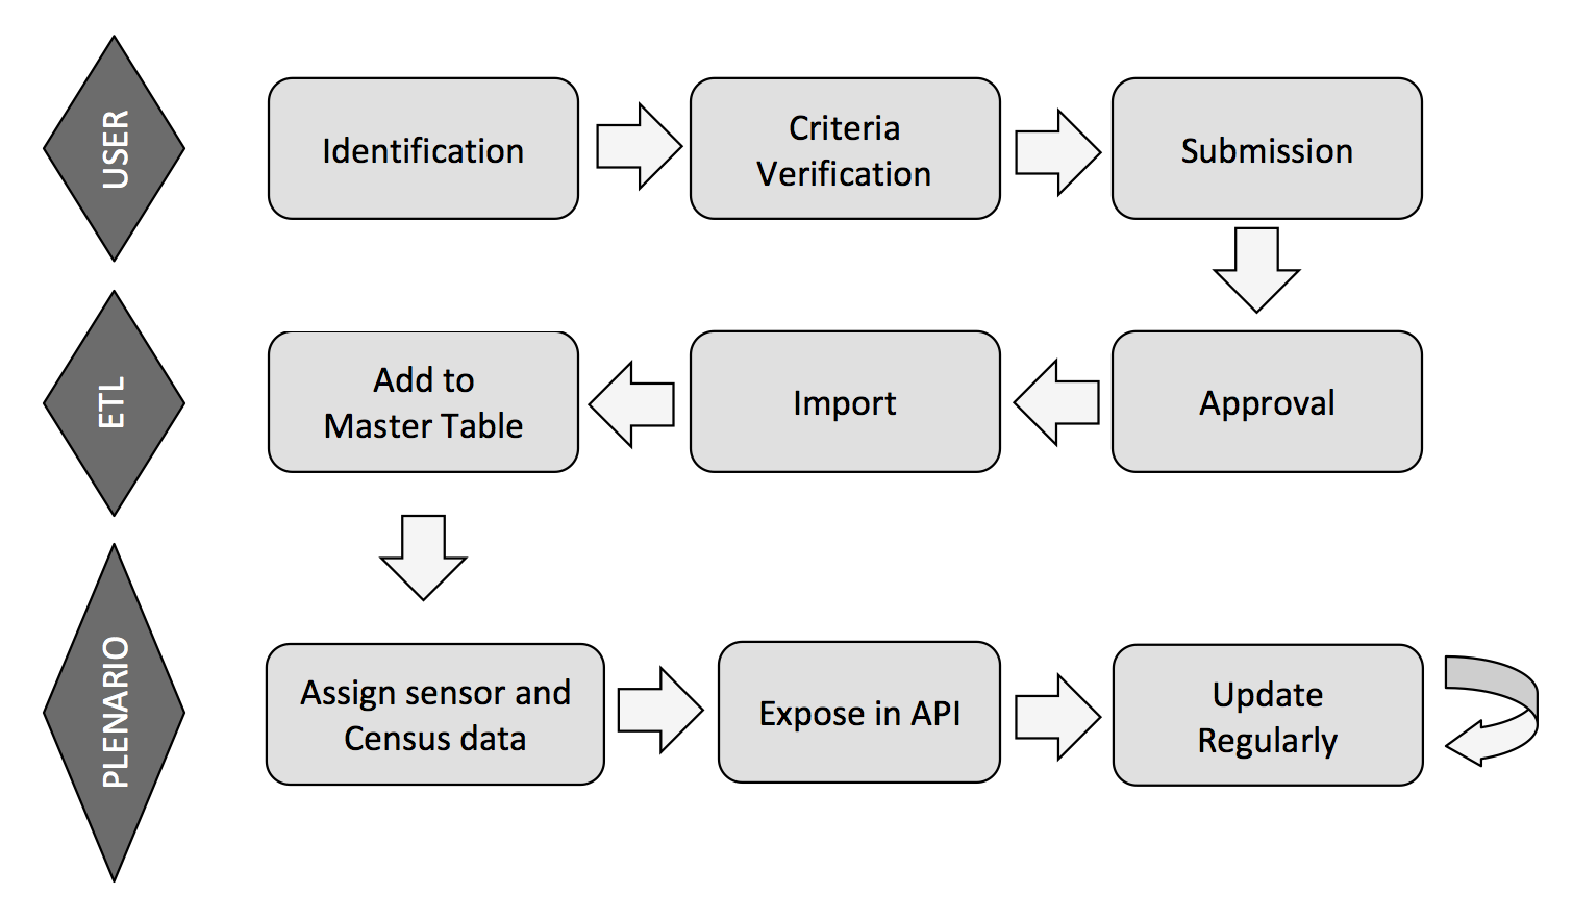
\includegraphics[scale=.45]{flowchart.pdf}
	\label{fig:flowchart}
	\caption{The path from identification of a dataset to making it available in the Plenario API. This process takes less than 24 hours for all but the largest datasets; we aim to accelerate it yet further.}
\end{figure}

\begin{figure}
	\centering
	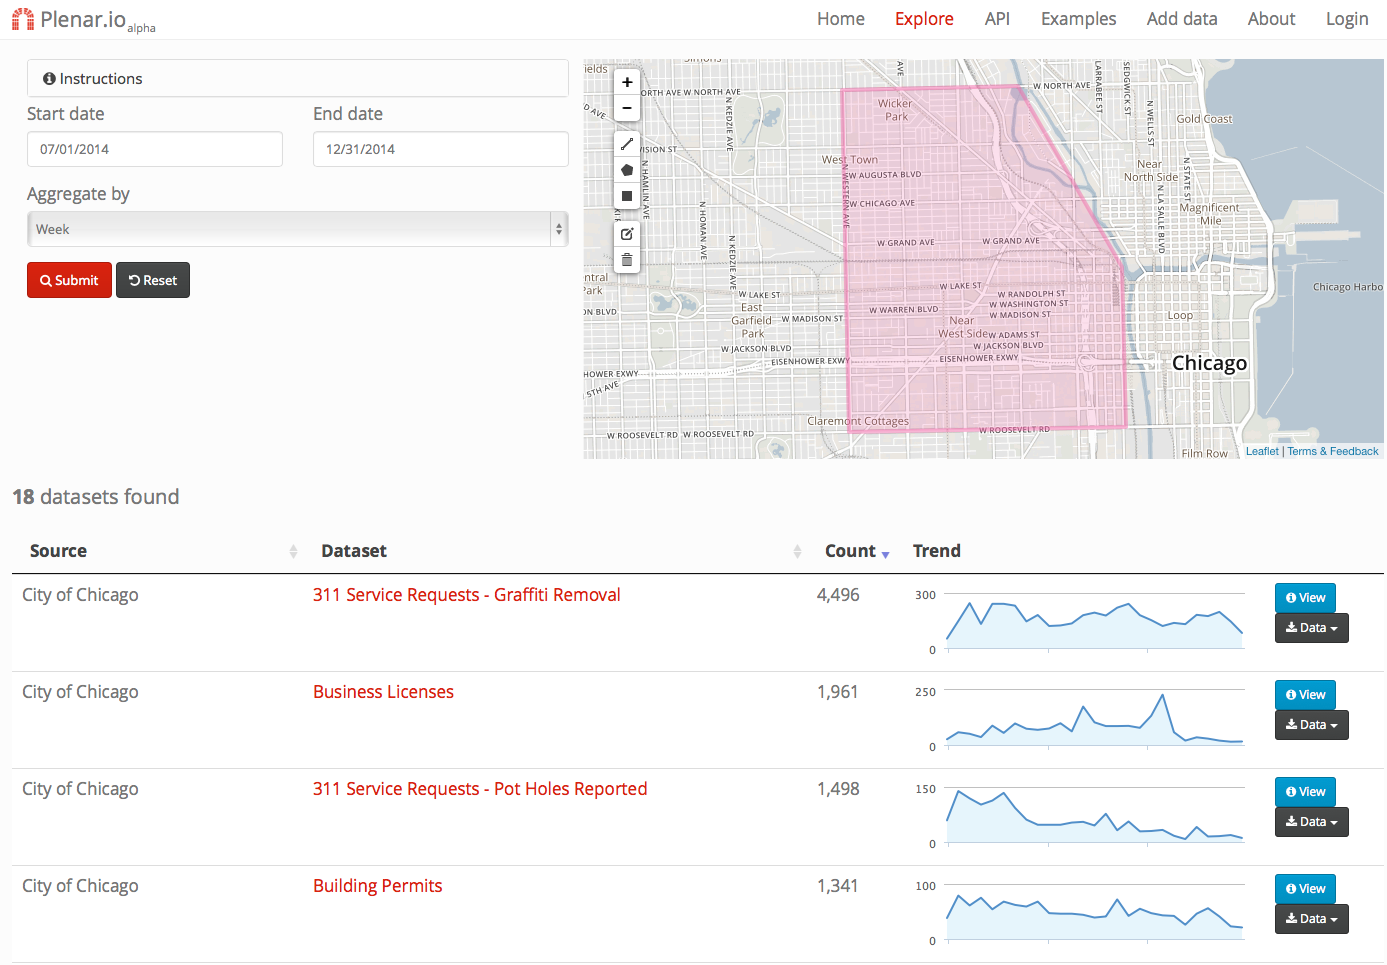
\includegraphics[scale=.25]{plenario_search_example.png}
	\label{fig:plenario-search-example}
	\caption{An example search using the Plenario portal. The search panel, at top, specifies the desired time period (the second half of 2014), aggregation (weekly), and spatial extent (the polygon). The results panel, truncated here to the first four of 18 matching data sources, includes not only basic metadata but also time series graphs as an indication of temporal dynamics.\ian{Is the term ``sparkline" appropriate here?}\vspace{.4cm}}
\end{figure}

\begin{figure}
	\centering
	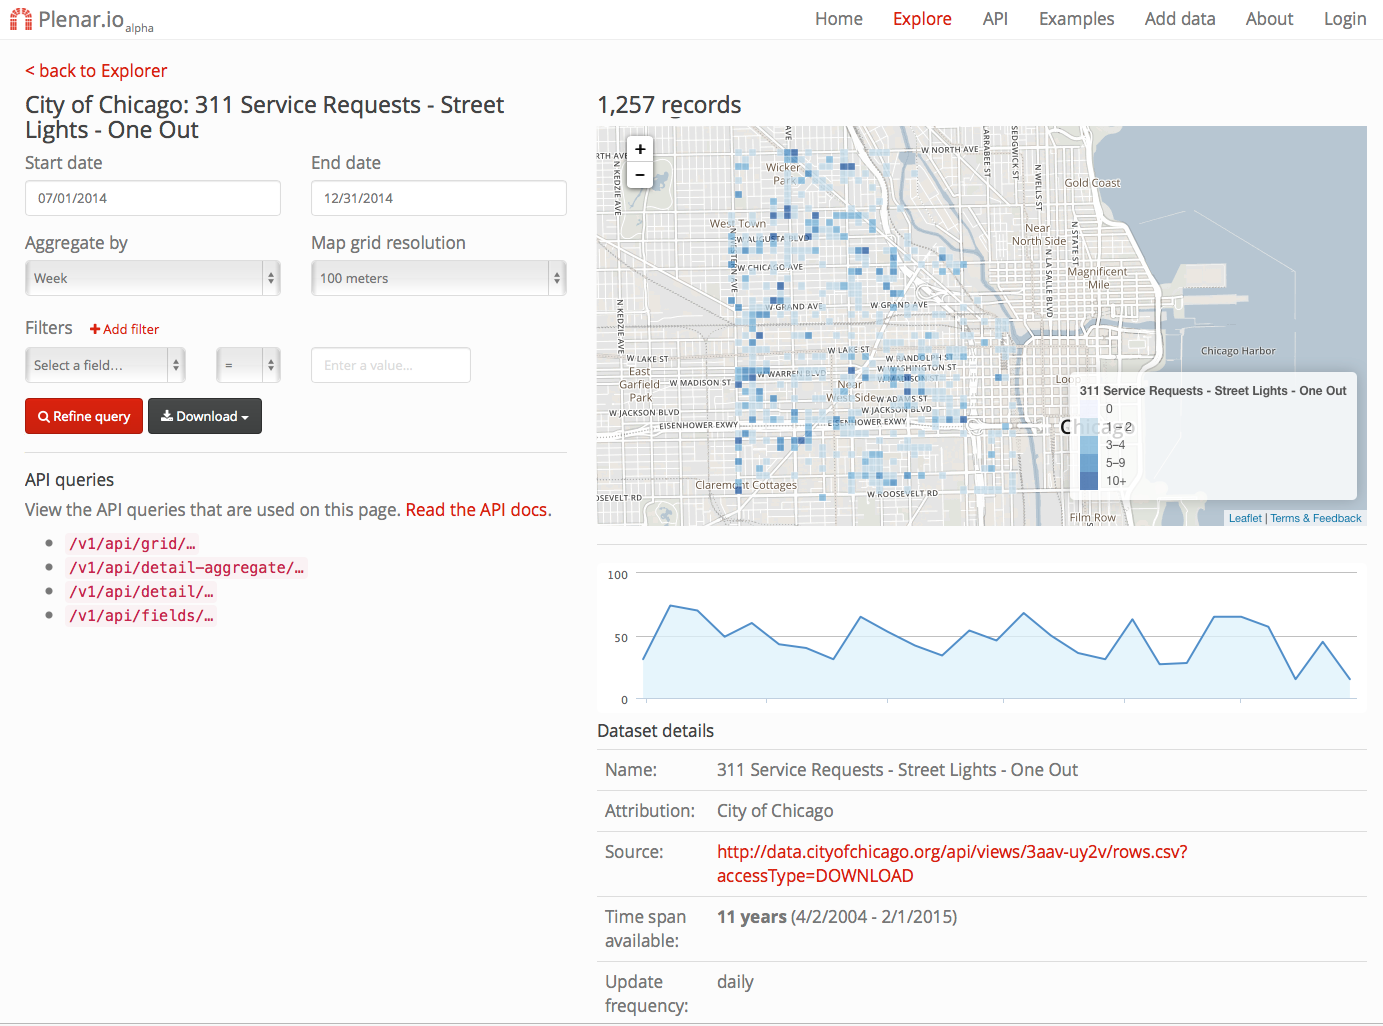
\includegraphics[scale=.25]{plenario_dataset_view.png}
	\label{fig:plenario-dataset-view}
	\caption{Plenario data set view. Selected from the first results screen, this view allows the user to view the spatial distribution of a given data set and provides links to the data and associated metadata. This screen also allows the user to change the temporal and spatial resolution of the query and to refine the data set by selecting and specifying values or ranges for individual record values.\vspace{.4cm}}
\end{figure}

\subsection{\textbf{Core Database: Single Spatio-Temporal Index and PostgreSQL Schema}}\label{sec:core-database}
Plenario achieves the workflow optimizations discussed in Section \ref{sec:context-objective} and illustrated in Figure \ref{fig:plenario-workflow} by organizing all records using common spatial and temporal indices in the Master Table (Figure \ref{fig:db-schema}). This approach has several important implications. 

First, data is automatically organized in an intuitive and coherent manner that can be easily searched and accessed by the user. In addition to API access, Plenario includes a portal interface (Figure \ref{fig:plenario-search-example}) that allows users to search for datasets by drawing polygons or paths on a map and selecting start and end dates. 

Second, data is organized, and can be searched for and accessed, without relying upon user knowledge of the existence of the data or its sources. Any point or polygon, and any time period, can be associated with data from multiple datasets, from multiple government agencies or organizations. This data can then be returned as a result of a search without the user needing to specify the data source. Thus, for example, a query for data points from Midtown Manhattan during June 2013 will return data from the City of New York, New York State, federal government, and numerous local or national organizations and surveys, including sources of which the user is unaware. 

The third implication is that data for any arbitrary geography can be readily organized as a time series containing counts (or other variables) of observations in each contained dataset. Plenario enables one-click download of such time series matrices---instant snapshots of a geography over time---with any temporal resolution from hours to decades. Plenario thus eliminates the tedious work of data compilation and aggregation along identical temporal and spatial units and allows users to begin simple analyses immediately.

\begin{figure}
	\centering
		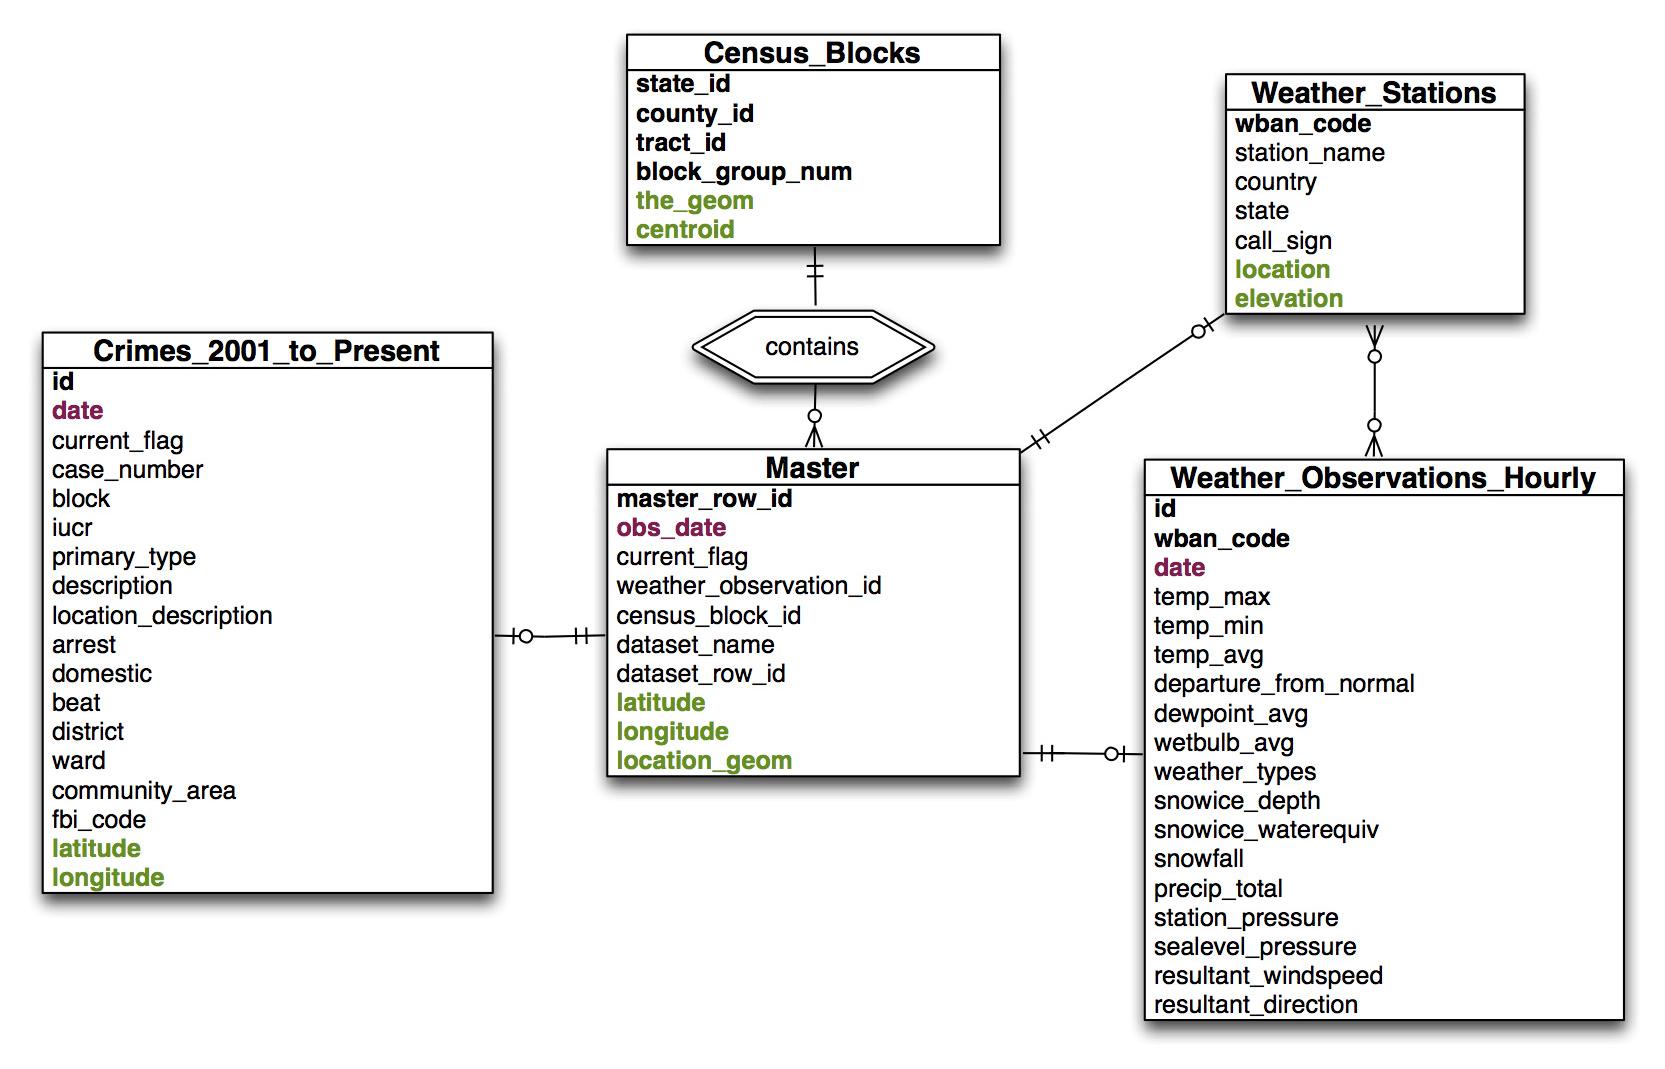
\includegraphics[scale=.45]{db_schema.pdf}
	\label{fig:db-schema}
	\caption{A subset of the PostgreSQL Schema used in the Plenario prototype. A sample dataset (on crime) feeds into the Master Table, which in turn links to spatial data (census blocks) and sensor data (weather observations) through the \texttt{census\_block\_id} and \texttt{weather\_observation\_id} fields. There is one row in the Master Table for every row in a source dataset like Crimes, but a many-to-many relationship exists between the Master Table and Census blocks or weather observations, because \ian{explain why}. Note that the \texttt{Weather\_Observations\_Hourly} table (which contains no spatial information) is filtered through the \texttt{Weather\_Stations} table (which contains no temporal information)\ian{I don't think that readers will necessarily understand the significance of the last sentence? Explain why some words are green?}. \vspace{.4cm}}
\end{figure}

\subsection{\textbf{Special Cases: Commonly Used Data Sets}}\label{sec:commonly-used-datasets}
Plenario was optimized to support not only particular data sets related to a specific topic but to enable investigations in the context of widely used data sources such as weather and location shapefiles\ian{Unclear to me: text reads to me as saying ``weather shapefiles and location shapefiles"--is that what is meant?}, and aggregated census information. Once a dataset is imported and inserted into the Master Table, Plenario enriches it with other data relevant to the same geography, including sensor and location-specific data. Below we discuss \textit{sensor data} (time series such as weather) and \textit{local data}\ian{Seems an odd term--isn't all of your data ``local"?} (relatively static data about the geography), which are also shown in Figure \ref{fig:db-schema}.

\textit{Sensor data}, which records one or more variables at regular intervals in fixed locations, usually along a network with high coverage (such as weather stations), is important both for tracking environmental variables over time and for enhancing human-generated data (such as noise complaints) with objective recordings from the same time and location (such as noise levels). 

Weather data in particular is important to many questions about place, from healthcare studies to traffic or flooding analysis. We thus include NOAA hourly and daily weather weather station data as an integral element of the Master Table scheme. To date, we have loaded into Plenario all U.S.\ hourly and daily weather station data since 2011.
We also assign to every record in the Master Table the weather station that is closest to it; thus, we can respond to any query requesting weather information about a record by retrieving the observation from its ``nearest" weather station for the time closest to the record's timestamp. The process is efficient because all weather data is stored in only one place, and because the closest weather stations are pre-calculated when a dataset is imported. 

This integration of weather station data provides an initial example of how sensor data adds to the open data landscape.
Further plans for sensor data include incorporating data from the Array of Things \cite{moser_2015} project in Chicago, which will report measures such as air pollution and noise at a much higher resolution, both temporally (every 30-60 seconds) and spatially (sensors will be deployed throughout Chicago, with densities ranging from one per square block to one per square kilometer). This data source will further illustrate the value of sensor data to municipal open datasets, enabling investigations such as the spatial and temporal characteristics of air quality in context of vehicle flow and weather, or the interrelationships between hyperlocal weather and crime. 

\textit{Local data} refers to data aggregated at a regional (not individual) level\ian{So ``local" data is not local but regional? :-)} containing variables that are relatively static over time, such as demographic data and local economic data. The University of Chicago implementation of Plenario\ian{This phrasing is confusing, as previously we have said there is one code implementation, and then multiple instances. Do you mean ``The Chicago Instance," to be consistent with later phrasing?} incorporates a prototypical example of local data, which is data from the United States Census: every row in the Master Table is coded with its FIPS Census block ID, which allows for easy enhancement with open data from other sources tied to that Census block, Census tract, county, state, etc., all of which can be determined from the Census block ID. 

\subsection{Components and AWS Implementation}
Plenario is built entirely from open source tools and is released under the MIT license. All code is in a GitHub repository \cite{plenario-github}, making the platform easy to fork and clone. Source datasets remain under their original license; most are released under the MIT license or are unlicensed.\ian{The first and second sentences is about the code, I presume. The third sentence is about data, which presumably various across Instances. Is this statement about the Chicago Instance?}

The platform is built as a PostgreSQL and PostGIS geospatial relational database. SQL Alchemy \cite{sqlalchemy} is used as the object relational mapper with the GeoAlchemy~2 extension. The web application with API was developed using Flask \cite{flask}, with mapping capabilities provided by Leaflet \cite{leaflet} and Open Street Map \cite{openstreetmap}. The ETL process uses Celery \cite{celery} for logging, and Redis \cite{redis} is available for caching support when high loads are anticipated. 

We host Plenario on Amazon Web Services (AWS)'s Elastic Cloud Compute (EC2) infrastructure. We currently use four virtual servers within a Virtual Private Cloud (VPC): one web server, one database server, one ETL worker server, and one gateway server. Due to its elastic nature, the EC2 server resources can be upgraded in real time as traffic load and data footprint increase. For larger deployments, the database server can be sharded and replicated for more capacity using the AWS Relational Database Service (RDS). Amazon Machine Images (AMI) can be used to snapshot the various server configurations for easy re-deployability.

For data integrity and redundancy, every raw dataset processed by the Plenario ETL worker is saved as a snapshot and stored on Amazon's Simple Storage Service (S3). This allows for data integrity checks, ETL fault tolerance and history tracking on every dataset Plenario ingests.

There are several ways for the community to use Plenario: a user can fork the GitHub code to develop a separate project, copy the entire project via a machine image on AWS, or feed data into the web portal supported by the University of Chicago at http://plenar.io. All of these modalities of use have been seen since Plenario's alpha launch in September 2014, including a repurposing of the core API to power the City of San Francisco's Sustainable Systems Framework initiative as detailed below. 

The web portal interface described above is in fact an application that accesses a Plenario instance running on AWS, via the Plenario API. This modular approach enables other front-end frameworks to be built to use the API, ranging from custom mobile and web applications (of which http://plenar.io is an example) to a complex analytics system such as WindyGrid, which uses commercial mapping and user interface software such as ESRI.

\section{Plenario Use Cases and Early Lessons Learned}
We have reviewed key features that the Plenario project was designed to provide for researchers, government employees, developers, journalists, and citizen users. Here we present several examples of where Plenario is being used today to support social and economic science research (the Chicago Plenario instance) and community engagement on urban sustainability, resilience, and livability goals (the San Francisco Plenario instance). 

\subsection{\textbf{Supporting Research: The Chicago Instance}}\label{chicago-instance}
The Chicago Instance, active at {\tt http://plenar.io}, is focused, as the name suggests, on the City of Chicago, but also incorporates data from other cities. 
The data that it contains have been selected to support research into urban science and computational approaches to public policy, as identified through the US-RCN;
they include data from open data portals operated by the City of Chicago, Cook County, State of Illinois, federal government, and also other data sets from hundreds of separate government departments such as the Illinois Department of Transportation, Chicago Department of Public Health, National Oceanic and Atmospheric Administration (NOAA), and U.S. Census Bureau.\ian{(1) Seems like it would be good to say how many datasets, how many data points? [I see some of this is below.] (2) The wording seems to imply that there are datasets from hundreds of departments, implying ``hundreds" of datasets. But below you say 150?}

This broad collection of data, when combined with Plenario's data discovery interfaces, allow researchers, journalists, and residents to rapidly identify datasets that interest them regardless of the original source. For example, Goldstein leads a team investigating the interrelationship between local weather and violent crime, which involves all of the base sensor and local data described in Section~\ref{sec:commonly-used-datasets} as well as urban crime data, 311 service call data, and other data sets.

As the Chicago instance has grown from dozens of data sets to over 150, we have found that Plenario's automatic data set summary feature has led users to identify a range of previously undetected data quality problems. For example, a single error in the date field is immediately apparent when a summary suggests that Plenario contains data from prehistoric times, or far into the future. We intend to incorporate consistency checks to flag obvious errors of this kind (such as impossible dates), but we note that not all errors are  readily flagged by algorithms. The very nature of data is that errors and holes are inevitable. Thus it will be important to not only work with data providers to fix obvious errors but to provide Plenario users with mechanisms to discover and flag errors. 

With goals to expand the Chicago instance to thousands of data sets, the Plenario team is also beginning to analyze the scalability of the Master Table approach and of our specific database implementation approach.

\subsection{\textbf{Enabling Community-Driven Urban Sustainability, Resilience, and Livability: The San Francisco Instance}}\label{san-francisco-instance}
The Plenario platform has also  been deployed experimentally as part of the City of San Francisco's Sustainable Development initiative \cite{sf-sustainable-systems}. This project has motivated important Plenario enhancements, including support for additional data types such as geographical information in the form of ESRI shapefiles. It has also spurred the development of new features to enable the use of Plenario as a community ``dashboard,'' whereby the visual interface is the primary use. (In contrast, the Chicago Instance is mostly used to refine and export data for advanced data analytics.) Several enhancements driven by the San Francisco implementation have already been incorporated into the core Plenario code base; others will be incorporated after further evaluation in the San Francisco instance.

The San Francisco instance contains datasets pertaining to a wide variety of sustainability indices, ranging from community structures accessibility to green space, canopy cover, water consumption, and energy use. The ability to discover and access such datasets instantly via spatial-temporal queries greatly empowers institutions and communities to assess the status quo and plan future efforts in sustainable development\ian{Any evidence for this assertion?}. In particular, the framework is to be used in the sustainable development of the South of Market (SoMa) ecodistrict.

The data needed for the applications that the San Francisco Instance is designed to support are highly heterogeneous in both content and form. For example, quantifying access to green spaces---the vicinity of parkland to residents---requires analysis of geographic information regarding the location and shape of each park, which cannot be treated simply as a point in space. Similarly, a community center is an entity that exists over a certain time span, in contrast to much place-based urban data such as crime or inspections, which are ``events'' that each occur at a specific instant.  
To incorporate these and other types of data, we extended Plenario's database schema and added new ETL functions. We also defined and developed efficient implementations of new query types, to support questions such as ``What is the average distance for residents of a given area to the closest farmer's market, at any point in time and in a given range\ian{What is a ``range"?}?''

The San Francisco Plenario instance is also exploring approaches\ian{Who is exploring these things? Presumably not the instance itself, unless Plenario has acquired AI?} to supporting a mix of open and sensitive data. As with the Census data in the Chicago instance, some San Francisco data is not public and is thus carefully aggregated to protect privacy. One algorithm that is commonly used for utilities datasets is the ``15/15 rule,'' which requires that no aggregation sample may contain less than 15 data points, and any point in any aggregation sample cannot represent more than 15\% of the measure for that sample. (The ``15/15 Rule'' was adopted by the California Public Utilities Commission in Decision D.97-10-031.) The methodology being explored in the San Francisco project is for the ``providers'' of the Plenario instance to securely host the raw data, executing the query- and data-specific privacy-preserving aggregations as a function of the particular search, view, and/or data export process.\ian{I find it unclear here as to whether this is work being done by the Chicago Plenario team, by SF people on a fork of the Plenario code, or completely separately.}

\section{Lessons, Challenges, and Opportunities}\label{sec:challenges}
Experience with the two large Plenario instances just described has identified challenges that must be addressed to move Plenario from an alpha platform to a fully supported and sustainable resource. We discuss these challenges in three groups: data, scaling, and architecture. 

\subsection{\textbf{Data Issues}}
Data is often collected in quite different ways across jurisdictions, because every local government has different goals in mind. Even datasets with similar purposes, such as 311 service requests or food safety inspection reports, can rarely be merged across jurisdictions, effectively limiting research to a focus on one particular city rather than incorporating and studying multiple cities at once. These barriers can exist at the metadata level (different variables recorded), in the resolution of the data (spatial and temporal), and even at the level of individual data points and fields (semantics and ontology). For example, a crime classified as ``assault'' in New York City crime data would be classified as a ``battery'' in Chicago crime data, which may mislead a researcher attempting to compare violent crime in the two cities or to compile a large dataset of crime in the United States. Furthermore, the definitions of ``assault" and ``battery" are not identical. 

We also encounter the common challenge of poor data quality and documentation. Because all data in Plenario ultimately refers to a source dataset hosted by a municipality, the remedy is limited to either cleaning the data upon insertion into Plenario or providing feedback to the data providers. Data cleaning at insertion accelerates availability of higher quality data, in comparison to relying on data providers, but also requires that the platform understand in each case what is ``correct.'' Ultimately we want to encode the policies to be followed for each data source and data set into the ETL process in a similar fashion to the update frequency.

A final data challenge is that many data sets do not define unique IDs to records. Thus, we cannot updating datasets incrementally, but must instead perform a full refresh of an entire dataset when new data becomes available. This approach increases load; more importantly, it can also introduce data consistency issues\ian{Why?} that can impact applications, particularly those aimed at real-time capabilities. 

\subsection{\textbf{Scaling Issues}}
The enormity of the open data landscape and the rapid pace with which open datasets are being released led us to design Plenario for scalability from the start.
Nevertheless, we have encountered scaling problems as our Master Table grows to billions of rows. 
We have explored a variety of solutions to these problems, such as partitioning the table along the temporal index, with mixed results. In particular, the number of NOAA hourly observations for all 2,200+ weather stations since 1997 in the United States was deemed too large to import in its entirety if we were to maintain a reliably responsive API. To work around this limitation, we only imported observations from weather stations within a certain radius of each dataset's bounding box, and then only since 2011.\ian{Presumably here you mean ``each dataset that is in the Chicago Instance at present," and thus as new datasets are added, we need to load more? Also, I added the mention of 2011 as that was mentioned above.}

The sensor data also contributes to scaling challenges. Although the closest weather station to every record is identified upon insertion into the Master Table, the platform executes the join\ian{which join?} at the time of request rather than as part of the insertion process. This join has significant impact on query performance; however, the alternative of precomputing the join would exacerbate scaling issues with the Master Table by making it extremely wide. Furthermore, sensor data needs to be spatially smoothed to avoid sharp boundaries in the data such as when two neighboring weather stations record significantly different values for a given variable\ian{This statement seems inconsistent with earlier statement that you select the nearest station for each record?}. To reduce computational load, we thus organize sensor data spatially using a Voronoi diagram \cite{voronoi_1908} without spatial smoothing.

\subsection{\textbf{Architecture and Data Semantics Issues}}
Plenario's original purpose as a platform for spatio-temporal data discovery and exploration brings into question how to map variables with ill-defined or uncertain locations in ``space'' and ``time.'' For example, should 311 data reflect the location of the caller or the location of the problem reported? How should the location of non-spatial crimes, like fraud or online crimes, be reported? How should Plenario represent records missing a spatial or temporal value? How can unstructured data be supported---especially when the location and datestamp of such data are uncertain?

We have also encountered challenges with respect to how to treat data with limited spatial and temporal resolution. For instance, how do we present city budget data that covers an entire city for the period of one year-{}-and make this data discoverable in typical user searches? Should a query across multiple years return multiple city budgets, only those wholly contained in the temporal arguments, or none at all? How should shapes like parks, streets, and parcel lots be dated? Some of these challenges are being highlighted in the San Francisco Plenario instance, as discussed earlier.

Ultimately these challenges suggest exploration into the optimal approach to support the integration of spatial/temporal data with data that is primarily ``entity'' based. In some cases, such as with census data, spatial and temporal mapping can be done in concert with data aggregation as is necessary for privacy protection. In other cases, particularly with organizations whose data includes internal private data about businesses and individuals, such mapping is less straightforward. Plenario currently supports questions such as ``where were the automobile accidents in mid-town Manhattan during heavy rainstorms in 2014'' but is not organized in order to refine this query to show only those accidents involving cars greater than 10 years old, or male drivers aged 18-24.

Finally, Plenario is currently designed as a portal for open data, which is only a subset of data useful for urban science and research, policy development, or many areas of improved urban operations. There are known solutions to challenges of multiple levels of authorization, and it will be important to integrate these solutions into the platform. The San Francisco Plenario instance supports sensitive data by aggregation at the time of query, presenting the aggregated data to the end user. The Chicago Plenario instance\ian{It would probably be good to be consistent as to whether write the ``Chicago Instance," ``Chicago Plenario Instance," ``Chicago instance," or ``Chicago Plenario instance," etc.} uses pre-aggregated census data, eliminating the need to aggregate at query time. While the latter approach improves query performance and reduces the sensitivity of the data stored in Plenario, it also requires that the aggregation algorithm be defined a priori. But in practice, different aggregation schemes may be more or less optimal for different types of inquiry.

\section{Conclusions and a Plenario Roadmap}
We have begun to develop a 12-18 month roadmap based on input from early users. We are developing a rigorous set of performance scaling tests that we will use to explore the architecture issues noted above. This exploration may motivate us to revisit various design decisions, from the underlying database to the Master Table. We are also considering various features requested by researchers, such as automated time series analysis to identify correlations between datasets. This feature could be used, for example, to identify subsets of 311 data that are lagged by violent crime in various city neighborhoods. 

Of particular interest to many place-based investigations is the identification of urban ``areas'' that function as units. Traditional boundaries such as neighborhoods or districts often do not reflect the underlying social or economic structure, in part because many such boundaries were drawn generations in the past and/or through political processes. The rapidly expanding variety of data being integrated into Plenario creates new opportunities to understand the factors that differentiate neighborhoods and to use spatial units defined by current data, not solely by a 20\textsuperscript{th} (or 19\textsuperscript{th}) century surveyor's pen. Concurrently, support for place-based research will require more powerful tools for specifying spatial data aggregation (Plenario already provides flexibility in temporal aggregation) to address the Modifiable Area Unit Problem \cite{wong_2009}: that is, the fact that the results of spatial analysis are often highly dependent on the spatial units used.

Today's open data landscape largely resembles the Internet of the 1980s when data was shared through anonymous file transfer servers, which were useful only to those with inside knowledge of their locations and contents. The advent of HTTP and web browsers led to today's powerful search and integration capabilities---including those that Plenario uses to import data! An overarching objective of the Plenario project is to ensure that these benefits extend to open data.
The first step toward this vision has been to implement the Plenario platform as a means to reduce or eliminate many of the challenges of working with open data, beginning with discovery, exploration, and integration across many sources. As we address these challenges, and the number of innovative applications of open data grows, we hope to see governments increasingly incentivized to release data. We also hope to reduce the need for governments to develop custom data portals. By providing the basic tools required to start extracting insight and return on investment from their data, we will \ian{???}. By building and encouraging a collaborative open data ecosystem at every stage, from identifying datasets to building third-party tools, Plenario helps push the full potential of this movement closer to realization. 

\section*{Acknowledgments}
The Plenario project is funded by the John D. and Catherine T. MacArthur Foundation and the National Science Foundation via an NSF Early-Concept Grant for Exploratory Research (EAGER) for software development (award number 1348865), while the interaction capabilities were driven by the Urban Sciences Research Coordination Network, created with an NSF Building Community and Capacity for Data-Intensive Research in the Social, Behavioral, and Economic Sciences and in Education and Human Resources (BCC-SBE/EHR) award.




\begin{thebibliography}{1}

\bibitem{maksimovic_2011}
Maksimovic, M.D.; Veljkovic, N.Z.; Stoimenov, L.V., ``Platforms for open government data,'' Telecommunications Forum (TELFOR), 2011 19th, vol., no., pp.1234,1237, 22-24 Nov. 2011. doi: 10.1109/TELFOR.2011.6143774

\bibitem{windygrid}
``Chicago's WindyGrid: Taking Situational Awareness to a New Level.'' \url{http://datasmart.ash.harvard.edu/news/article/chicagos-windygrid-taking-situational-awareness-to-a-new-level-259} [Accessed July 7, 2015]

\bibitem{urbanccd}
The Urban Center for Computation and Data, at the Computation Institute of the University of Chicago and Argonne National laboratory. \url{http://www.urbanccd.org} [Accessed July 7, 2015]

\bibitem{us-rcn}
NSF 1244749, ``BCC-SBE: An Urban Sciences Research Coordination Network for Data-Driven Urban Design and Analysis. \ PI Catlett, C., University of Chicago. 2012-2015.

\bibitem{socrata}
\url{http://www.socrata.com/} [Accessed July 7, 2015]

\bibitem{ckan}
\url{http://ckan.org/} [Accessed July 7, 2015]

\bibitem{plenario-github}
\url{https://github.com/UrbanCCD-UChicago/plenario} [Accessed July 7, 2015]

\bibitem{moser_2015}
Moser, W, ``What Chicago's `Array of Things' Will Actually Do,'' Chicago Magazine, January 27, 2014. See also \url{http://ArrayofThings.github.io} [Accessed July 7, 2015]

\bibitem{sqlalchemy}
\url{http://www.sqlalchemy.org/} [Accessed July 7, 2015]

\bibitem{flask}
\url{http://flask.pocoo.org/} [Accessed July 7, 2015]

\bibitem{leaflet}
\url{http://leafletjs.com/} [Accessed July 7, 2015]

\bibitem{openstreetmap}
\url{http://www.openstreetmap.org/about} [Accessed July 7, 2015]

\bibitem{celery}
\url{http://www.celeryproject.org/} [Accessed July 7, 2015]

\bibitem{redis}
\url{http://redis.io/} [Accessed July 7, 2015]

\bibitem{sf-sustainable-systems}
``The Sustainable Development Program.'' \url{http://www.sf-planning.org/index.aspx?page=3051} [Accessed July 7, 2015]

\bibitem{voronoi_1908}
Voronoi, G., Nouvelles applications des param\'etres continus \'a la th\'eorie des formes quadratiques. Deuxi\`eme m\'emoiure: recherches sur les parall\`eloedes primitifs, J. reine angew. Math. 134, 198-287 (1908)

\bibitem{wong_2009}
Wong, D., ``The modifiable areal unit problem (MAUP)'', In Fotheringham, A Stewart; Rogerson, Peter. \textit{The SAGE handbook of spatial analysis}. pp.~105--124 (2009)

\end{thebibliography}







\end{document}